\begin{center}
	ĐỀ ÔN TẬP KIỂM TRA GIỮA HỌC KỲ I – MÔN VẬT LÝ 11\\
	Thời gian làm bài: 50 phút \\
	(Không kể thời gian phát đề)\\
\end{center}
\section{Trắc nghiệm \textit{(6,0 điểm)}}
\ANSMCQ{
	\begin{center}
		\begin{tabular}{|m{2.8em}|m{2.8em}|m{2.8em}|m{2.8em}|m{2.8em}|m{2.8em}|m{2.8em}|m{2.8em}|m{2.8em}|m{2.8em}|}
			\hline
			1D & 2A & 3B & 4A & 5C & 6A & 7D & 8B & 9C & 10B\\
			\hline
			11D & 12B & 13D & 14C & 15A & 16A & 17C & 18A & 19B & 20D\\
			\hline
		\end{tabular}
\end{center}}
\begin{enumerate}[label=\bfseries Câu \arabic*:]
	\item Khi vật thực hiện một dao động tương ứng với pha dao động sẽ thay đổi một lượng 
	\begin{mcq}(4)
		\item $\SI{0}{\radian}$.
		\item $\xsi{\dfrac{\pi}{2}}{\radian}$.
		\item $\xsi{\pi}{\radian}$.
		\item $\xsi{2\pi}{\radian}$.
	\end{mcq}
\hideall{
\textbf{Đáp án D.}
}


\item Đơn vị đo của tần số dao động trong hệ đơn vị SI là 
\begin{mcq}(4)
	\item $\si{\hertz}$.
	\item $\si{\second}$.
	\item $\si{\centi\meter}$.
	\item $\si{\meter}$.
\end{mcq}
\hideall{
\textbf{Đáp án A.}
}

\item Độ dịch chuyển cực đại của vật tính từ vị trí cân bằng gọi là
\begin{mcq}(4)
	\item li độ dao động.
	\item biên độ dao động.
	\item tần số góc.
	\item pha ban đầu.
\end{mcq}
\hideall{
\textbf{Đáp án B.}
}

\item Trong các dao động được mô tả dưới đây, dao động nào được xem là dao động tuần hoàn? 
\begin{mcq}
	\item Dao động của con lắc đồng hồ khi đang hoạt động. 
	\item Dao động của chiếc thuyền trên mặt sông. 
	\item Dao động của quả bóng cao su đang nảy trên mặt đất. 
	\item Dao động của dây đàn sau khi được gảy.
\end{mcq}
\hideall{
\textbf{Đáp án A.}\\
Dao động tuần hoàn là dao động mà trạng thái chuyển động được lặp lại như cũ sau những khoảng thời gian bằng nhau xác định.
}

\item Một vật dao động điều hoà trên trục $Ox$. Hình bên là đồ thị biểu diễn sự phụ thuộc của li độ $x$ vào thời gian $t$. Tần số góc của dao động là
\begin{center}
	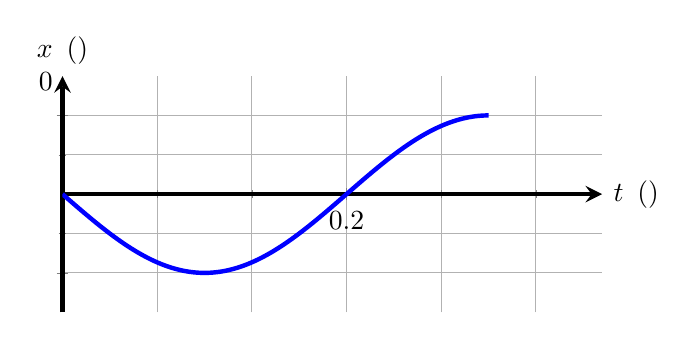
\begin{tikzpicture}  
		\begin{axis}[  ultra thick,
			xmin=0,  
			xmax=0.38,  
			xtick={0,0.2,0.4},
			ytick={-2,0,2},
			minor x tick num=2,
			minor y tick num=1,
			ymin=-3,  
			ymax=3, 
			y=0.5cm,
			samples=300,
			yticklabels=\empty,
			axis lines=center, 
			grid style={step=1, color=gray!60!white},
			grid=both,
			xlabel=$t\ \left(\si{\second}\right)$, 
			ylabel=$x\ \left(\si{\centi\meter}\right)$, 
			every axis y label/.style={at=(current axis.above origin),anchor=south},  
			every axis x label/.style={at=(current axis.right of origin),anchor=west},  ]
			\addplot [ultra thick, blue, smooth, domain=0:0.3] {2*cos(deg(5*pi*x+pi/2))}; 
		\end{axis}  
		\node[label={[left]90:0}] at (0,2.8){};
	\end{tikzpicture}
\end{center}
\begin{mcq}(4)
	\item $\SI{10}{\radian/\second}$.
	\item $\xsi{10\pi}{\radian/\second}$.
	\item $\xsi{5\pi}{\radian/\second}$.
	\item $\SI{5}{\radian/\second}$.
\end{mcq}
\hideall{
\textbf{Đáp án C.}\\
Chu kì dao động của vật $T=\SI{0.4}{\second}$.\\
Tần số góc dao động:
$$\omega=\dfrac{2\pi}{T}=\xsi{5\pi}{\radian/\second}.$$
}

\item Các nhà thực nghiệm đo được tần số dao động của một hệ gồm thanh silicon siêu nhỏ có virus dính trên đó đang thực hiện dao động là $\SI{2.87E14}{\hertz}$. Tần số góc của hệ dao động trên bằng bao nhiêu? 
\begin{mcq}(4)
	\item $\SI{1.80E15}{\radian/\second}$.
	\item $\SI{3.48E15}{\radian/\second}$.
	\item $\SI{2.18E14}{\radian/\second}$.
	\item $\SI{4.57E14}{\radian/\second}$.
\end{mcq}
\hideall{
\textbf{Đáp án A.}\\
Tần số góc của dao động:
$$\omega=2\pi f=\SI{1.80E15}{\radian/\second}.$$
}

\item Một vật dao động điều hoà trên trục $Ox$. Vận tốc của vật
\begin{mcq}(2)
	\item luôn có giá trị không đổi.
	\item luôn có giá trị dương.
	\item là hàm bậc hai của thời gian.
	\item biến thiên điều hoà theo thời gian.
\end{mcq}
\hideall{
\textbf{Đáp án D.}\\
Vận tốc của vật dao động điều hoà biến thiên điều hoà theo thời gian.
}

\item Khi nói về dao động điều hòa của một vật, phát biểu nào sau đây đúng?
\begin{mcq}
	\item Khi vật ở vị trí biên, gia tốc của vật bằng không.
	\item Vectơ gia tốc của vật luôn hướng về vị trí cân bằng.
	\item Vectơ vận tốc của vật luôn hướng về vị trí cân bằng.
	\item Khi đi qua vị trí cân bằng, vận tốc của vật bằng không.
\end{mcq}
\hideall{
\textbf{Đáp án B.}
}

\item Khi tiến hành thí nghiệm khảo sát vị trí vật nặng của con lắc lò xo đang dao động bằng cách sử dụng thước thẳng, bạn học sinh thấy rằng vật nặng dao động từ vị trí $\SI{1}{\centi\meter}$ đến vị trí $\SI{11}{\centi\meter}$ trên thước. Biên độ dao động của vật nặng trong con lắc lò xo là 
\begin{mcq}(4)
	\item $\SI{10}{\centi\meter}$.
	\item $\SI{6}{\centi\meter}$.
	\item $\SI{5}{\centi\meter}$.
	\item $\SI{12}{\centi\meter}$.
\end{mcq}
\hideall{
\textbf{Đáp án C.}\\
Biên độ dao động của vật nặng trong con lắc lò xo:
$$A=\dfrac{\ell_\text{max}-\ell_\text{min}}{2}=\SI{5}{\centi\meter}.$$
}

\item Trong dao động điều hoà, khoảng thời gian mà vật thực hiện được 1 dao động toàn phần gọi là
\begin{mcq}(4)
	\item biên độ,
	\item chu kì.
	\item tần số.
	\item pha ban đầu.
\end{mcq}
\hideall{
\textbf{Đáp án B.}\\
Khoảng thời gian mà vật thực hiện được 1 dao động toàn phần gọi là chu kì dao động.
}

\item Một bạn học sinh quan sát thấy con lắc trong đồng hồ quả lắc thực hiện được 20 dao động trong 30 giây. Dao động của con lắc trong đồng hồ này có đặc điểm nào sau đây? 
\begin{mcq}(2)
	\item Dao động điều hoà, tần số là $\SI{1.5}{\hertz}$.
	\item Dao động điều hoà, tần số là $\SI{0.7}{\hertz}$.
	\item Dao động tuần hoàn, tần số là $\SI{1.5}{\hertz}$.
	\item Dao động tuần hoàn, tần số là $\SI{0.7}{\hertz}$.
\end{mcq}
\hideall{
\textbf{Đáp án D.}\\
Dao động của con lắc đồng hồ là dao động tuần hoàn với tần số
$$f=\dfrac{N}{\Delta t}=\dfrac{20}{\SI{30}{\second}}\approx\SI{0.67}{\hertz}.$$
}

\item Hai vật dao động điều hoà có đồ thị li độ - thời gian như hình vẽ. Phát biểu nào sau đây mô tả đúng tính chất của hai vật?
\begin{center}
	\includegraphics[width=0.6\linewidth]{../figs/D11-2-1}
\end{center}
\begin{mcq}(2)
	\item Hai vật dao động cùng tần số, cùng pha. 
	\item Hai vật dao động cùng tần số, vuông pha. 
	\item Hai vật dao động khác tần số, cùng pha. 
	\item Hai vật dao động khác tần số, vuông pha.
\end{mcq}
\hideall{
\textbf{Đáp án B.}\\
Dựa vào đồ thị li độ - thời gian, ta nhận thấy hai vật dao động cùng tần số.\\
Tại thời điểm $t=0$, vật 2 qua VTCB theo chiều dương. Sau khoảng thời gian $\Delta t=\dfrac{T}{4}$ vật 1 có cùng trạng thái dao động với vật 2 ở thời điểm $t=0$. Suy ra, độ lệch pha giữa hai dao động:
$$\Delta \varphi=\dfrac{\Delta t}{T}\cdot2\pi=\xsi{\dfrac{\pi}{2}}{\radian}.$$
}

\item Đồ thị li độ thời gian của một vật dao động điều hoà được thể hiện như hình vẽ. Phương trình dao động của vật là
\begin{center}
	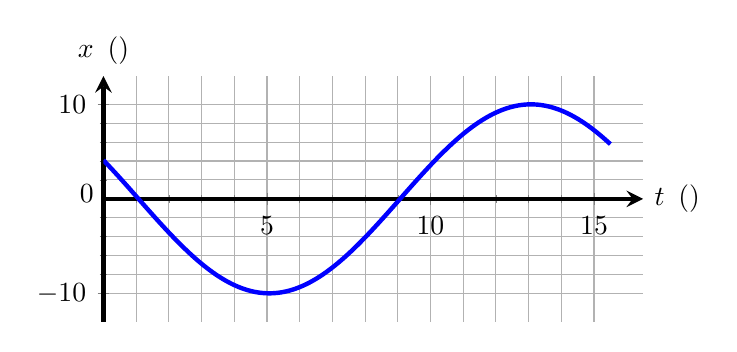
\begin{tikzpicture}  
		\begin{axis}[  ultra thick,
			xmin=0,  
			xmax=16.5,  
			xtick={0,5,10,15},
			ytick={-10,0,10},
			minor x tick num=4,
			minor y tick num=4,
			ymin=-13,  
			ymax=13, 
			y=0.12cm,
			samples=300,
			axis lines=center, 
			grid style={step=1, color=gray!60!white},
			grid=both,
			xlabel=$t\ \left(\si{\second}\right)$, 
			ylabel=$x\ \left(\si{\centi\meter}\right)$, 
			every axis y label/.style={at=(current axis.above origin),anchor=south},  
			every axis x label/.style={at=(current axis.right of origin),anchor=west},  ]
			\addplot [ultra thick, blue, smooth, domain=0:15.5] {10*cos(deg(pi*x/8+1.15))}; 
		\end{axis}  
		\node[label={[left]90:0}] at (0,1.5){};
	\end{tikzpicture}
\end{center}
	\begin{mcq}(2)
		\item $x=\xsi{10\cos\left(16t+1,37\right)}{\centi\meter}$.
		\item $x=\xsi{10\cos\left(\dfrac{\pi}{8}t-1,18\right)}{\centi\meter}$.
		\item $x=\xsi{10\cos\left(16t-1,37\right)}{\centi\meter}$.
		\item $x=\xsi{10\cos\left(\dfrac{\pi}{8}t+1,18\right)}{\centi\meter}$.
	\end{mcq}
\hideall{
\textbf{Đáp án D.}\\
Chu kì dao động của vật:
$$\dfrac{T}{2}=\SI{13}{\second}-\SI{5}{\second}\Rightarrow T=\SI{16}{\second}$$
Tần số góc dao động:
$$\omega=\dfrac{2\pi}{T}=\xsi{\dfrac{\pi}{8}}{\radian/\second}$$
Tại thời điểm $t=\SI{5}{\second}$, vật đang ở vị trí biên âm, pha dao động của vật lúc này
$$\varphi=\omega t+\varphi_0=\xsi{\pi}{\radian}\Rightarrow \varphi_0=\varphi-\omega t=\xsi{\pi}{\radian}-\left(\xsi{\dfrac{\pi}{8}}{\radian/\second}\right)\cdot\left(\SI{5}{\second}\right)=\xsi{\dfrac{3\pi}{8}}{\radian}\approx\SI{1.18}{\radian}.$$
Phương trình dao động của vật:
$$x=\xsi{10\cos\left(\dfrac{\pi}{8}t+1,18\right)}{\centi\meter}.$$
}

\item Một vật dao động điều hoà với chu kì $\SI{2}{\second}$, biên độ $\SI{10}{\centi\meter}$. Khi vật cách vị trí biên $\SI{4}{\centi\meter}$ thì tốc độ của nó bằng
\begin{mcq}(4)
	\item $\SI{18.33}{\centi\meter/\second}$.
	\item $\SI{28.79}{\centi\meter/\second}$.
	\item $\SI{25.13}{\centi\meter/\second}$.
	\item $\SI{18.84}{\centi\meter/\second}$.
\end{mcq}
\hideall{
\textbf{Đáp án C.}\\
Tốc độ của vật khi cách vị trí biên $\SI{4}{\centi\meter}$ $\left(\left|x\right|=\SI{6}{\centi\meter}\right)$:
$$\left|v\right|=\omega\sqrt{A^2-x^2}=\left(\dfrac{\xsi{2\pi}{\radian}}{\SI{2}{\second}}\right)\sqrt{\left(\SI{10}{\centi\meter}\right)^2-\left(\SI{6}{\centi\meter}\right)^2}\approx\SI{25.13}{\centi\meter/\second}.$$
}

\item Một vật dao động điều hoà có gia tốc biến đổi theo thời gian $a=\xsi{8\cos\left(20t-\dfrac{\pi}{2}\right)}{\centi\meter/\second^2}$. Phương trình dao động của vật là
\begin{mcq}(2)
	\item $x=\xsi{0,02\cos\left(20t+\dfrac{\pi}{2}\right)}{\centi\meter}.$
	\item $x=\xsi{2\cos\left(20t-\dfrac{\pi}{2}\right)}{\centi\meter}.$
	\item $x=\xsi{4\cos\left(20t+\dfrac{\pi}{2}\right)}{\centi\meter}.$
	\item $x=\xsi{2\cos\left(20t+\dfrac{\pi}{2}\right)}{\centi\meter}.$
\end{mcq}
\hideall{
\textbf{Đáp án A.}\\
Biên độ dao động của vật:
$$A=\dfrac{a_\text{max}}{\omega^2}=\dfrac{\SI{8}{\centi\meter/\second^2}}{\left(\SI{20}{\radian/\second}\right)^2}=\SI{0.02}{\centi\meter}$$
Pha ban đầu của dao động:
$$\varphi_{0x}=\varphi_{0a}+\pi=\xsi{\dfrac{\pi}{2}}{\radian}.$$
Vậy phương trình dao động của vật $x=\xsi{0,02\cos\left(20t+\dfrac{\pi}{2}\right)}{\centi\meter}$.\\
}

\item Một chất điểm dao động điều hoà, gia tốc $a$ và li độ $x$ của chất điểm liên hệ với nhau bởi hệ thức $a=-4\pi^2x$, trong đó $a$ có đơn vị $\si{\centi\meter/\second^2}$; $x$ có đơn vị $\si{\centi\meter}$. Chu kì dao động bằng
\begin{mcq}(4)
	\item $\SI{1}{\second}$.
	\item $\SI{0.25}{\second}$.
	\item $\SI{0.5}{\second}$.
	\item $\SI{0.4}{\second}$.
\end{mcq}
\hideall{
\textbf{Đáp án A.}\\
Mối liên hệ giữa gia tốc và li độ của vật dao động điều hoà:
$$a=-\omega^2x\Rightarrow \omega=\xsi{2\pi}{\radian/\second}$$
$$\Rightarrow T=\dfrac{2\pi}{\omega}=\SI{1}{\second}.$$
}

\item Một vật dao động điều hoà trên trục $Ox$ với phương trình $x=\xsi{5\cos\left(4\pi t-\dfrac{\pi}{3}\right)}{\centi\meter}$. Khoảng thời gian ngắn nhất để vật đi từ li độ $x_1=\SI{-2.5}{\centi\meter}$ đến vị trí $x_2=\xsi{\dfrac{5\sqrt{3}}{2}}{\centi\meter}$ là
\begin{mcq}(4)
	\item $\xsi{\dfrac{5}{48}}{\second}$.
	\item $\xsi{\dfrac{5}{24}}{\second}$.
	\item $\xsi{\dfrac{1}{8}}{\second}$.
	\item $\xsi{\dfrac{3}{20}}{\second}$.
\end{mcq}
\hideall{
\textbf{Đáp án C.}\\
\begin{center}
	\begin{tikzpicture}
		\coordinate (O) at (0,0);
		\coordinate (A) at (240:3);
		\coordinate (B) at (330:3);
		\coordinate (D) at (5,0);
		\coordinate (E) at (-4,0);
		\draw[line width=1.0] (O) circle[radius=3];
		
		\draw [fill=cyan!20](330:3)--(0,0)--(240:3) arc (240:330:3)--cycle;
		\draw[-stealth, line width=1.0] (E) -- (D);
		\draw[-stealth, line width=1.0] (0,-4) -- (0,4);
		\tkzMarkRightAngle[size=0.3,color=blue](A,O,B);
		\draw[-stealth,thick,red] (O) -- (A);
		\draw[-stealth,thick,red] (O) -- (B);
		\draw[dashed] (A) -- ($(O)!(A)!(D)$);
		\draw[dashed] (B) -- ($(O)!(B)!(D)$);
		
		\fill   (O) circle[radius=2pt]  node [above left] {$O$};
		\fill   ($(O)!(A)!(D)$) circle[radius=2pt, color=teal];
		\fill   ($(O)!(B)!(E)$) circle[radius=2pt,color=teal];
		\fill   (3,0) circle[radius=2pt]  node [above right] {$5$};
		\fill   (-3,0) circle[radius=2pt]  node [above left] {$-5$};
		\node[label={[above]90:$x \left(\si{\centi\meter}\right)$}] at ($(D)-(0,0.2)$){};
		\node[label={[above]90:$-2,5$}] at ($(O)!(A)!(D)$){};
		\node[label={[above left]90:$\dfrac{5\sqrt{3}}{2}$}] at ($(O)!(B)!(D)$){};
	\end{tikzpicture}
\end{center}
Dựa vào vòng tròn lượng giác, thời gian ngắn nhất để vật đi từ vị trí $x_1=\SI{-2.5}{\centi\meter}$ đến vị trí $x_2=\xsi{\dfrac{5\sqrt{3}}{2}}{\centi\meter}$
 là
 $$\Delta t=\dfrac{T}{4}=\dfrac{1}{4}\cdot\dfrac{2\pi}{\omega}=\xsi{\dfrac{1}{8}}{\second}
.$$}

\item Một vật dao động điều hoà trên quỹ đạo dài $\SI{8}{\centi\meter}$. Tốc độ của vật khi qua vị trí cân bằng là $\xsi{0,4\pi}{\meter/\second}$. Gọi mốc thời gian là lúc vật đi qua vị trí $\xsi{2\sqrt{3}}{\centi\meter}$ theo chiều dương. Phương trình dao động của vật là
\begin{mcq}(2)
	\item $x=\xsi{4\cos\left(10\pi t-\dfrac{\pi}{6}\right)}{\centi\meter}$.
	\item $x=\xsi{4\cos\left(10\pi t+\dfrac{\pi}{6}\right)}{\centi\meter}$.
	\item $x=\xsi{2\cos\left(10\pi t-\dfrac{\pi}{6}\right)}{\centi\meter}$.
	\item $x=\xsi{2\cos\left(10\pi t+\dfrac{\pi}{6}\right)}{\centi\meter}$.
\end{mcq}
\hideall{
\textbf{Đáp án A.}\\
Biên độ dao động của vật
$$A=\dfrac{L}{2}=\SI{4}{\centi\meter}$$
Tần số góc dao động
$$\omega=\dfrac{v_\text{max}}{A}=\dfrac{\xsi{40\pi}{\radian/\second}}{\SI{4}{\centi\meter}}=\xsi{10\pi}{\radian/\second}$$
Chọn mốc thời gian lúc vật đi qua vị trí $\xsi{2\sqrt{3}}{\centi\meter}$ theo chiều dương. Pha ban đầu
$$\varphi_0=-\arccos\dfrac{x_0}{A}=-\xsi{\dfrac{\pi}{6}}{\radian}$$
}

\item Một vật dao động điều hoà trên trục $Ox$. Khi vật qua vị trí cân bằng thì tốc độ của nó là $\SI{20}{\centi\meter/\second}$. Khi vật có tốc độ là $\SI{10}{\centi\meter/\second}$ thì gia tốc của nó có độ lớn $\xsi{40\sqrt{3}}{\centi\meter/\second^2}$. Biên độ dao động của vật bằng
\begin{mcq}(4)
	\item $\SI{4}{\centi\meter}$.
	\item $\SI{5}{\centi\meter}$.
	\item $\SI{16}{\centi\meter}$.
	\item $\SI{8}{\centi\meter}$.
\end{mcq}
\hideall{
\textbf{Đáp án B.}\\
$$\dfrac{v^2}{v^2_\text{max}}+\dfrac{a^2}{a^2_\text{max}}=1\Rightarrow a_\text{max}=\SI{80}{\centi\meter/\second^2}$$
Biên độ dao động của vật:
$$A=\dfrac{v^2_\text{max}}{a_\text{max}}=\SI{5}{\centi\meter}.$$
}

\item Đồ thị động năng theo thời gian của một vật có khối lượng $\SI{0.4}{\kilogram}$ dao động điều hoà. Tại thời điểm ban đầu vật đang chuyển động theo chiều dương. Lấy $\pi^2=10$. Phương trình dao động của vật có dạng
\begin{center}
	\begin{tikzpicture}  
		\begin{axis}[  ultra thick,
			xmin=0,  
			xmax=1.2,  
			xtick={0,1.0},
			ytick={0,2},
			minor x tick num=5,
			minor y tick num=3,
			yticklabels=\empty,
			xticklabels=\empty,
			ymin=0,  
			ymax=2.5, 
			y=1.5cm,
			samples=300,
			axis lines=center, 
			grid style={step=1, color=gray!60!white},
			grid=both,
			xlabel=$t\ \left(\si{\second}\right)$, 
			ylabel=$W_\text{đ}\ \left(\si{\joule}\right)$, 
			every axis y label/.style={at=(current axis.above origin),anchor=south},  
			every axis x label/.style={at=(current axis.right of origin),anchor=west},  ]
			\addplot [ultra thick, blue, smooth, domain=0:1.0] {1+1*cos(deg(4*pi*x+pi/3))}; 
		\end{axis}  
		\node[label={[left]90:0}] at (0,0){};
		\node[label={[left]90:0,02}] at (0,2.9){};
		\node[label={[below]90:$\dfrac{1}{6}$}] at (1,-0.1){};
	\end{tikzpicture}
\end{center}
\begin{mcq}(2)
	\item $x=\xsi{5\cos\left(2\pi t+\dfrac{\pi}{3}\right)}{\centi\meter}$.
	\item $x=\xsi{10\cos\left(2\pi t+\dfrac{5\pi}{6}\right)}{\centi\meter}$.
	\item $x=\xsi{10\cos\left(2\pi t-\dfrac{5\pi}{6}\right)}{\centi\meter}$.
	\item $x=\xsi{5\cos\left(2\pi t-\dfrac{\pi}{3}\right)}{\centi\meter}$.
\end{mcq}
\hideall{
\textbf{Đáp án D.}\\
Chu kì dao động của động năng:
$$2T'=6\cdot\left(\xsi{\dfrac{1}{6}}{\second}\right)=\SI{1}{\second}\Rightarrow T'=\SI{0.5}{\second}$$
Chu kì dao động của vật:
$$T=2T'=\SI{1}{\second}$$
Ban đầu vật ở vị trí có $\dfrac{W_\text{đ}}{W}=\dfrac{\SI{0.015}{\joule}}{\SI{0.02}{\joule}}=\dfrac{3}{4}\Rightarrow W_\text{t}=\dfrac{W}{4}\Leftrightarrow x=\pm\dfrac{A}{2}$ và tốc độ đang giảm (đang chuyển động về vị trí biên).\\
Kết hợp với dữ kiện đề bài, ban đầu vật chuyển động theo chiều dương nên vị trí ban đầu của vật ứng với $x=\dfrac{A}{2}$.\\
Pha ban đầu của dao động:
$$\varphi_0=-\arccos\dfrac{x_0}{A}=\arccos\dfrac{1}{2}=-\xsi{\dfrac{\pi}{3}}{\radian}$$
Phương trình dao động của vật:
$$x=\xsi{5\cos\left(2\pi t-\dfrac{\pi}{3}\right)}{\centi\meter}.$$
}
\end{enumerate}
\section{Tự luận \textit{(4,0 điểm)}}
\begin{enumerate}[label=\bfseries Bài \arabic*:]
	\item Cho đồ thị vận tốc theo thời gian của một vật dao động điều hòa như hình vẽ. Biết rằng khối lượng của vật là $\SI{150}{\gram}$. Hãy xác định
	\begin{center}
		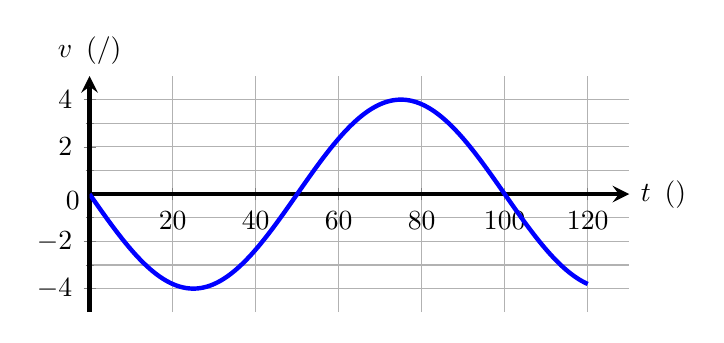
\begin{tikzpicture}  
			\begin{axis}[  ultra thick,
				xmin=0,  
				xmax=130,  
				xtick={0,20,40,60,...,120},
				ytick={-4,-2,0,2,4},
				minor x tick num=0,
				minor y tick num=1,
				ymin=-5,  
				ymax=5, 
				y=0.3cm,
				samples=300,
				axis lines=center, 
				grid style={step=1, color=gray!60!white},
				grid=both,
				xlabel=$t\ \left(\si{\milli\second}\right)$, 
				ylabel=$v\ \left(\si{\meter/\second}\right)$, 
				every axis y label/.style={at=(current axis.above origin),anchor=south},  
				every axis x label/.style={at=(current axis.right of origin),anchor=west},  ]
				\addplot [ultra thick, blue, smooth, domain=0:120] {4*cos(deg(0.02*pi*x+pi/2))}; 
			\end{axis}  
			\node[label={[left]90:0}] at (0,1.3){};
		\end{tikzpicture}
	\end{center}
	\begin{enumerate}[label=\alph*)]
		\item chu kì dao động của vật.
		\item biên độ dao động của vật.
		\item cơ năng của vật dao động.
		\item vị trí và gia tốc của vật tại thời điểm $\SI{100}{\milli\second}$.
	\end{enumerate}
\hideall{
\begin{enumerate}[label=\alph*)]
	\item Chu kì dao động của vật:
	$$T=\SI{100}{\milli\second}$$
	\item Tần số góc dao động:
	$$\omega=\dfrac{2\pi}{T}=\xsi{20\pi}{\radian/\second}$$
	Biên độ dao động của vật:
	$$A=\dfrac{v_\text{max}}{\omega}=\dfrac{\SI{4E2}{\centi\meter/\second}}{\xsi{20\pi}{\radian/\second}}\approx\SI{6.37}{\centi\meter}$$
	\item Cơ năng của vật dao động:
	$$W=W_\text{đ max}=\dfrac{1}{2}mv^2_\text{max}=\dfrac{1}{2}\cdot\left(\SI{0.15}{\kilogram}\right)\cdot\left(\SI{4}{\meter/\second}\right)^2=\SI{1.2}{\joule}$$
	\item Tại thời điểm $t=\SI{100}{\milli\second}$ vật có vận tốc bằng 0 và đang giảm $\Rightarrow$ vật ở vị trí biên dương $x=A=\SI{6.37}{\centi\meter}$.\\
	Gia tốc của vật lúc này:
	$$a=-\omega^2 x=-\left(\xsi{20\pi}{\radian/\second}\right)^2\cdot\left(\SI{6.37}{\centi\meter}\right)\approx\SI{25147.75}{\centi\meter/\second^2}.$$
\end{enumerate}

}
\item Quả lắc của đồng hồ cổ treo tường có tác dụng vận hành cho đồng hồ chạy đúng giờ.\\
\begin{minipage}[l]{0.55\textwidth}
	Cứ sau mỗi chu kì dao động của quả lắc, do sức cản và việc vận hành hệ thống bánh răng để các kim đồng hồ chạy nên nó tiêu hao năng lượng $\Delta E=\SI{0.100}{\milli\joule}$. Năng lượng này được lấy từ một quả tạ có trọng lượng $P=\SI{50.0}{\newton}$ treo trong hoặc ngoài đồng hồ.
	\begin{enumerate}[label=\alph*)]
		\item Vì sao sau một thời gian dài đồng hồ chạy thì quả tạ bị hạ thấp xuống và ta lại phải đưa nó lên cao?
		\item Nếu chạy trong thời gian $t=10\ \text{ngày}$ thì quả tạ sẽ giảm độ cao bao nhiêu mét? Biết trong 30 chu kì dao động của quả lắc thì kim giây chuyển động được một vòng.
	\end{enumerate}
\end{minipage}
\begin{minipage}[c]{0.05\textwidth}
	\
\end{minipage}
\begin{minipage}[l]{0.4\textwidth}
	\begin{center}
		\includegraphics[width=0.5\linewidth]{../figs/D11-2-2}
		\captionof{figure}{Hai quả tạ là nguồn năng lượng cung cấp để dao động của quả lắc không bị tắt (một quả dùng cho hệ thống chuông).}
	\end{center}
\end{minipage}
\hideall{
\begin{enumerate}[label=\alph*)]
	\item Quả tạ dự trữ năng lượng dưới dạng thế năng trọng trường. Mỗi chu kì dao động, thế năng này giảm dần đề bù cho phần năng lượng tiêu hao của quả lắc và hệ thống bánh răng. Do đó, độ cao quả tạ giảm dần.
	\item Mỗi phút, kim giây chuyển động hết 1 vòng và con lắc đồng hồ thực hiện 30 chu kì.\\
	Như vậy, số chu kì con lắc thực hiện được trong 10 ngày là:
	$$N=10 \cdot24\cdot\left(\SI{60}{\minute}\right)\cdot\left(30\ \text{chu kì/\si{\minute}}\right)=432000\ \text{chu kì}$$
	Tổng năng lượng tiêu hao trong 10 ngày:
	$$E=\left(432000\ \text{chu kì}\right)\cdot\left(\SI{0.100E-3}{\joule/\text{chu kì}}\right)=\SI{43.2}{\joule}$$
	Năng lượng tiêu hao này được bù bằng độ giảm thế năng trọng trường của quả tạ. Do đó, độ cao quả tạ bị giảm một đoạn:
	$$\Delta h=\dfrac{E}{P}=\dfrac{\SI{43.2}{\joule}}{\SI{50.0}{\newton}}=\SI{0.864}{\meter}.$$
	
\end{enumerate}

}
\end{enumerate}